\section{Experiments}
\label{sec:exp}

Based on Section \ref{sec:model} and \ref{sec:trainer}, we have
implemented the proposed {\sppan} model in both Python and C++ that can
run on a single machine. We also developed an parallel C++ version of
{\sppan} model based on Map-reduce.

In this section, we provide evaluation experiments for the performance
of the {\sppan} model. More specifically, we use the Python version
{\sppan} model, and compared its performance with a baseline method
and two Nonnegative Matrix Factorization based methods provided by
nimfa Python library \cite{ZitnikZ12}:

\begin{itemize} \itemsep -2pt
\item {\em Baseline}: The baseline method is giving prediction simply
  based on the average value in the training set.
\item {\em LSNMF}: It is based on Alternating nonnegative least
  squares matrix factorization using projected gradient method for
  subproblems\cite{lin2007projected}.
\item {\em NMF}: It is based on Standard nonnegative matrix
  factorization with Euclidean / Kullback-Leibler update equations and
  Frobenius / divergence / connectivity cost
  functions\cite{lee2001algorithms, brunet2004metagenes}.
\end{itemize}

To provide more interpretable experiment results and for data privacy
considerations, we show the performance result of NMF, LSNMF and
{\sppan} as their relative performance to the baseline method in all
the following subsections. The results of the evaluation experiments
show salient advantages of {\sppan} model compare to those two NMF
based methods:

\begin{itemize} \itemsep -2pt
\item {} The matrix factorization based methods LSNMF and NMF are not
  handling the present extreme sparse CTR data set very well. Their
  prediction accuracy is even worse than the baseline method.
\item {} In terms of the training and testing error (Root-mean-square
  deviation), {\sppan} model performs more than $65\%$ and $40\%$ better
  than the matrix factorization based methods, and around $60\%$ and
  $30\%$ better than the baseline method.
\item {} {\sppan} model has a normal error distribution centered at 0,
  which means a balanced estimation; while LSNMF and NMF have biased
  error distributions that are constantly under estimating.
\end{itemize}

\subsection{Data Description}
\label{sec:data_desc}
Our evaluation experiments are performed on a click-through rate (CTR)
dataset generated from Google Adsense, which was collected with
appropriate end-user license agreement and was fully anonymized
without any retrievable personally identifiable information.

The CTR data set can be considered as a 2D matrix shown in Figure
\ref{fig:problem-as-matrix}, where each row represents an advertiser
and each column represent a target keyword. The value of each matrix
entry in Figure \ref{fig:problem-as-matrix} is the weekly average
click-through rate (CTR) that we observed for the corresponding
advertiser on that specific keyword. The whole dataset is extremely
sparse because there are hundreds of thousands of different keywords
but advertisers usually only target at several of them. To be more
specific, the dataset contains more than 400k different advertisers
(number of rows) and 500k keywords (number of columns), but more than
$99.98\%$ entries in the dataset matrix are missing.

Because the two Nonnegative Matrix Factorization based methods
provided by nimfa cannot handle the entire CTR dataset ($400k \times
500k$ sparse matrix) on a single machine, we also generated a
sub-sampled version of data set in addition to the original one. To
generate the sub-sampled dataset, we go through each entry in the
original dataset and only keep that entry with specified
probability. If all the entry for a row (advertiser) or column
(keyword) are dropped, we simply remove that row (advertiser) or
column (keyword) all together. In Table \ref{tab:data}, we summarized
the basic information of both the $10\%$ sub-sampled version and
original data set, including the number of different advertisers,
keywords and known CTR entries. It can be seen that both datasets are
extremely sparse with more than $99.98\%$ of the entries missing.


\begin{table}[!ht]
\centering
\begin{tabular}{|c|c|c|}
  \hline	\hline
  Dataset & whole & $10\%$ sub-sampled\\ \hline
  Advertisers & $\sim 400K$ & $\sim 76K$  \\ 
  Keywords & $\sim 511K$ & $\sim 73K$  \\ 
  Known CTR entries &  $\sim 21M$ & $\sim 2M$ \\ \hline
\end{tabular}
\caption{Basic Information}
\label{tab:data}
\end{table}

\subsection{Evaluation}
To compare the estimation performance between LSNMF, NMF and {\sppan}
methods, we separate the sub-sampled CTR dataset described in Section
\ref{sec:data_desc} into a $95\%$ training set and a $5\%$ testing set
through random selecting. The experiment is very straightforward. For
each method, we use the $95\%$ training set for model training, and
test the model on estimating the entry values in the $5\%$ testing
set.

\begin{figure}[!ht]
  \centering
  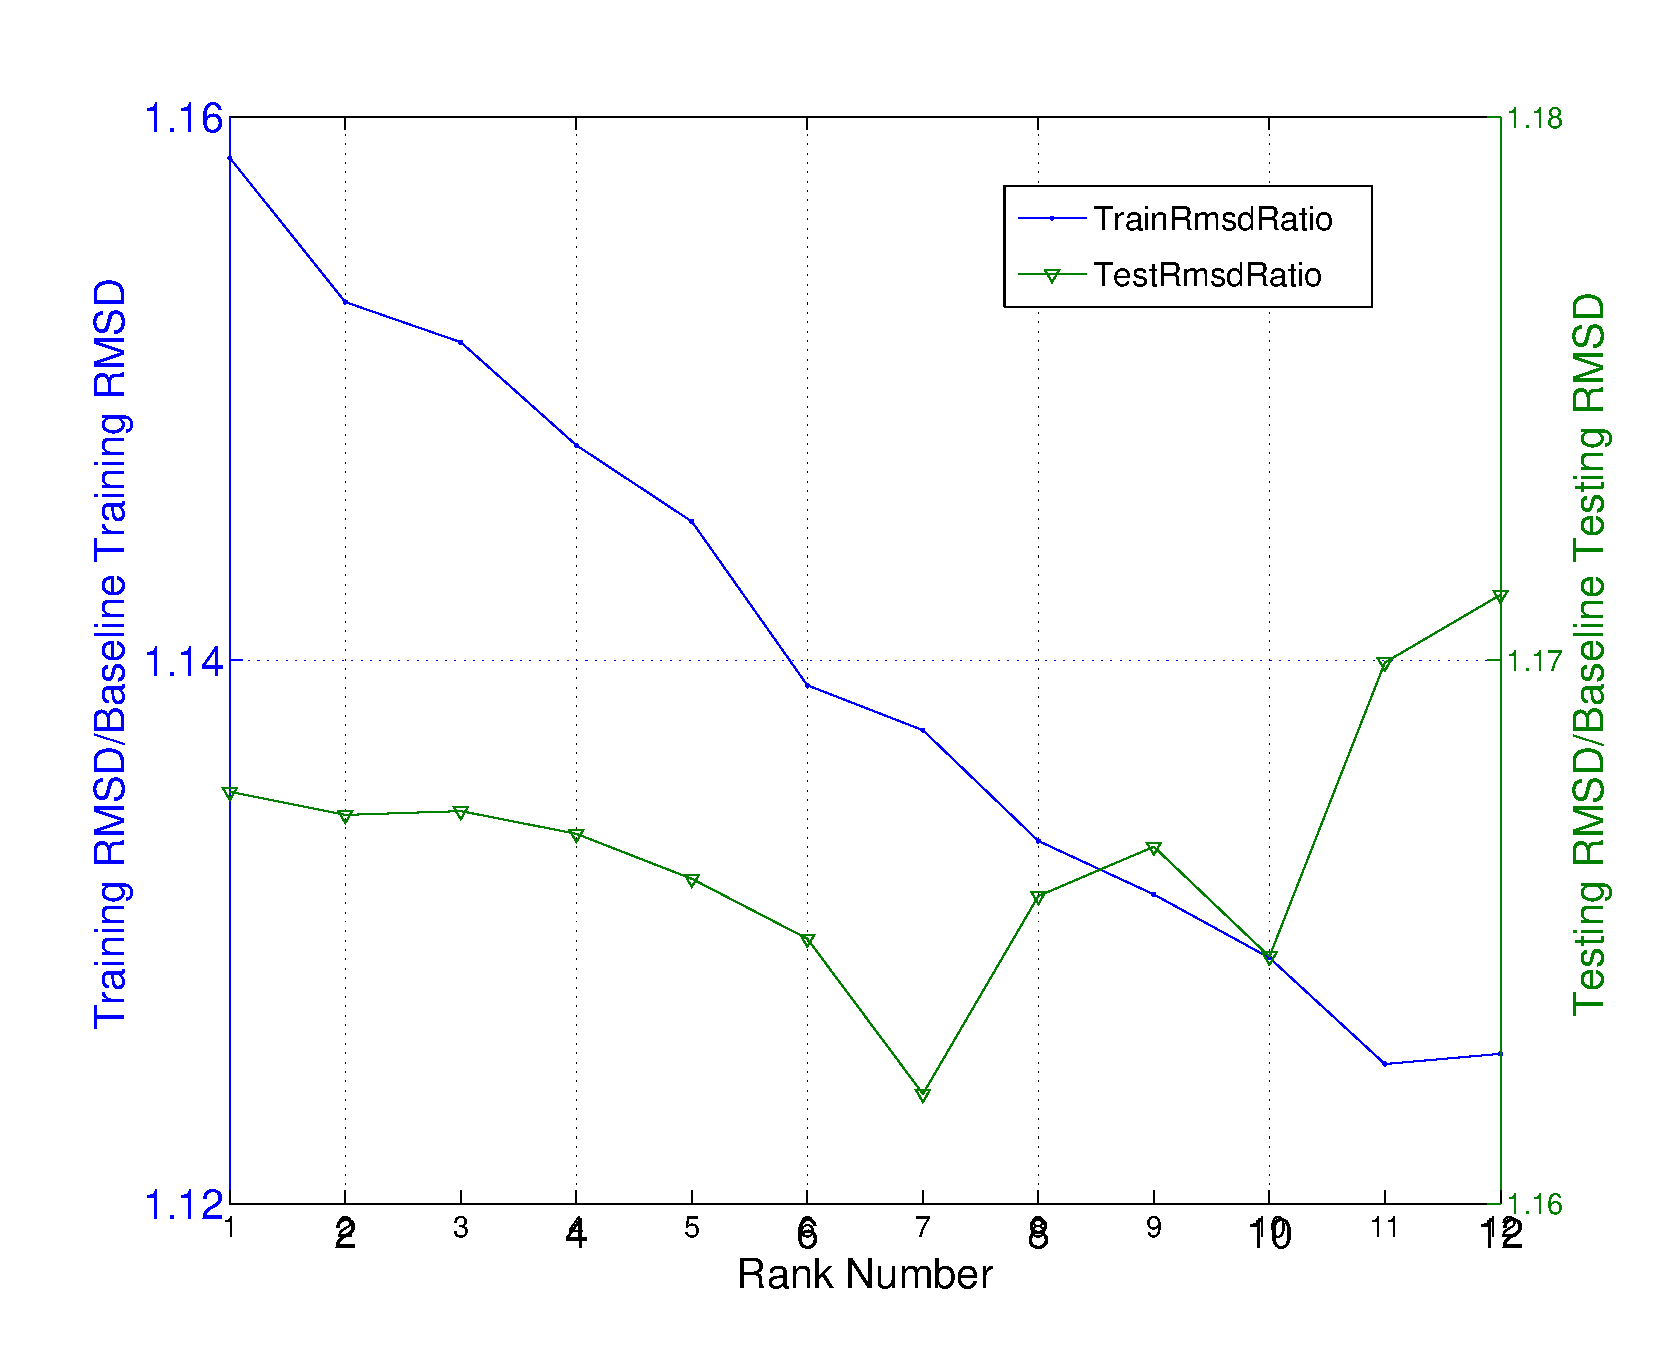
\includegraphics[width=0.4\textwidth]{figures/learning_curve_lsnmf_subsample_relative.eps}
  \caption{LSNMF: Relative Training/Testing Error Versus Rank Number}
  \label{fig:lsnmf_learning}
\end{figure}

For the Nonnegative Matrix Factorization based method LSNMF and NMF,
the Factorization Matrix Rank need to be specified before training the
model. Using a higher rank number often means a more complicated
matrix model, which is more powerful to represent a dataset but with
higher risk of over-fitting. On the other hand, using a lower rank
number means a simpler matrix model, which is less possible to be
over-fitted but might be too simple to represent the data set. We have
tried rank number from 1 to 12 for both LSNMF and NMF methods, their
results are very similar. The result training error and testing error
versus rank parameter of LSNMF method is shown in Figure
\ref{fig:lsnmf_learning}.

\begin{figure}[!ht]
  \centering
  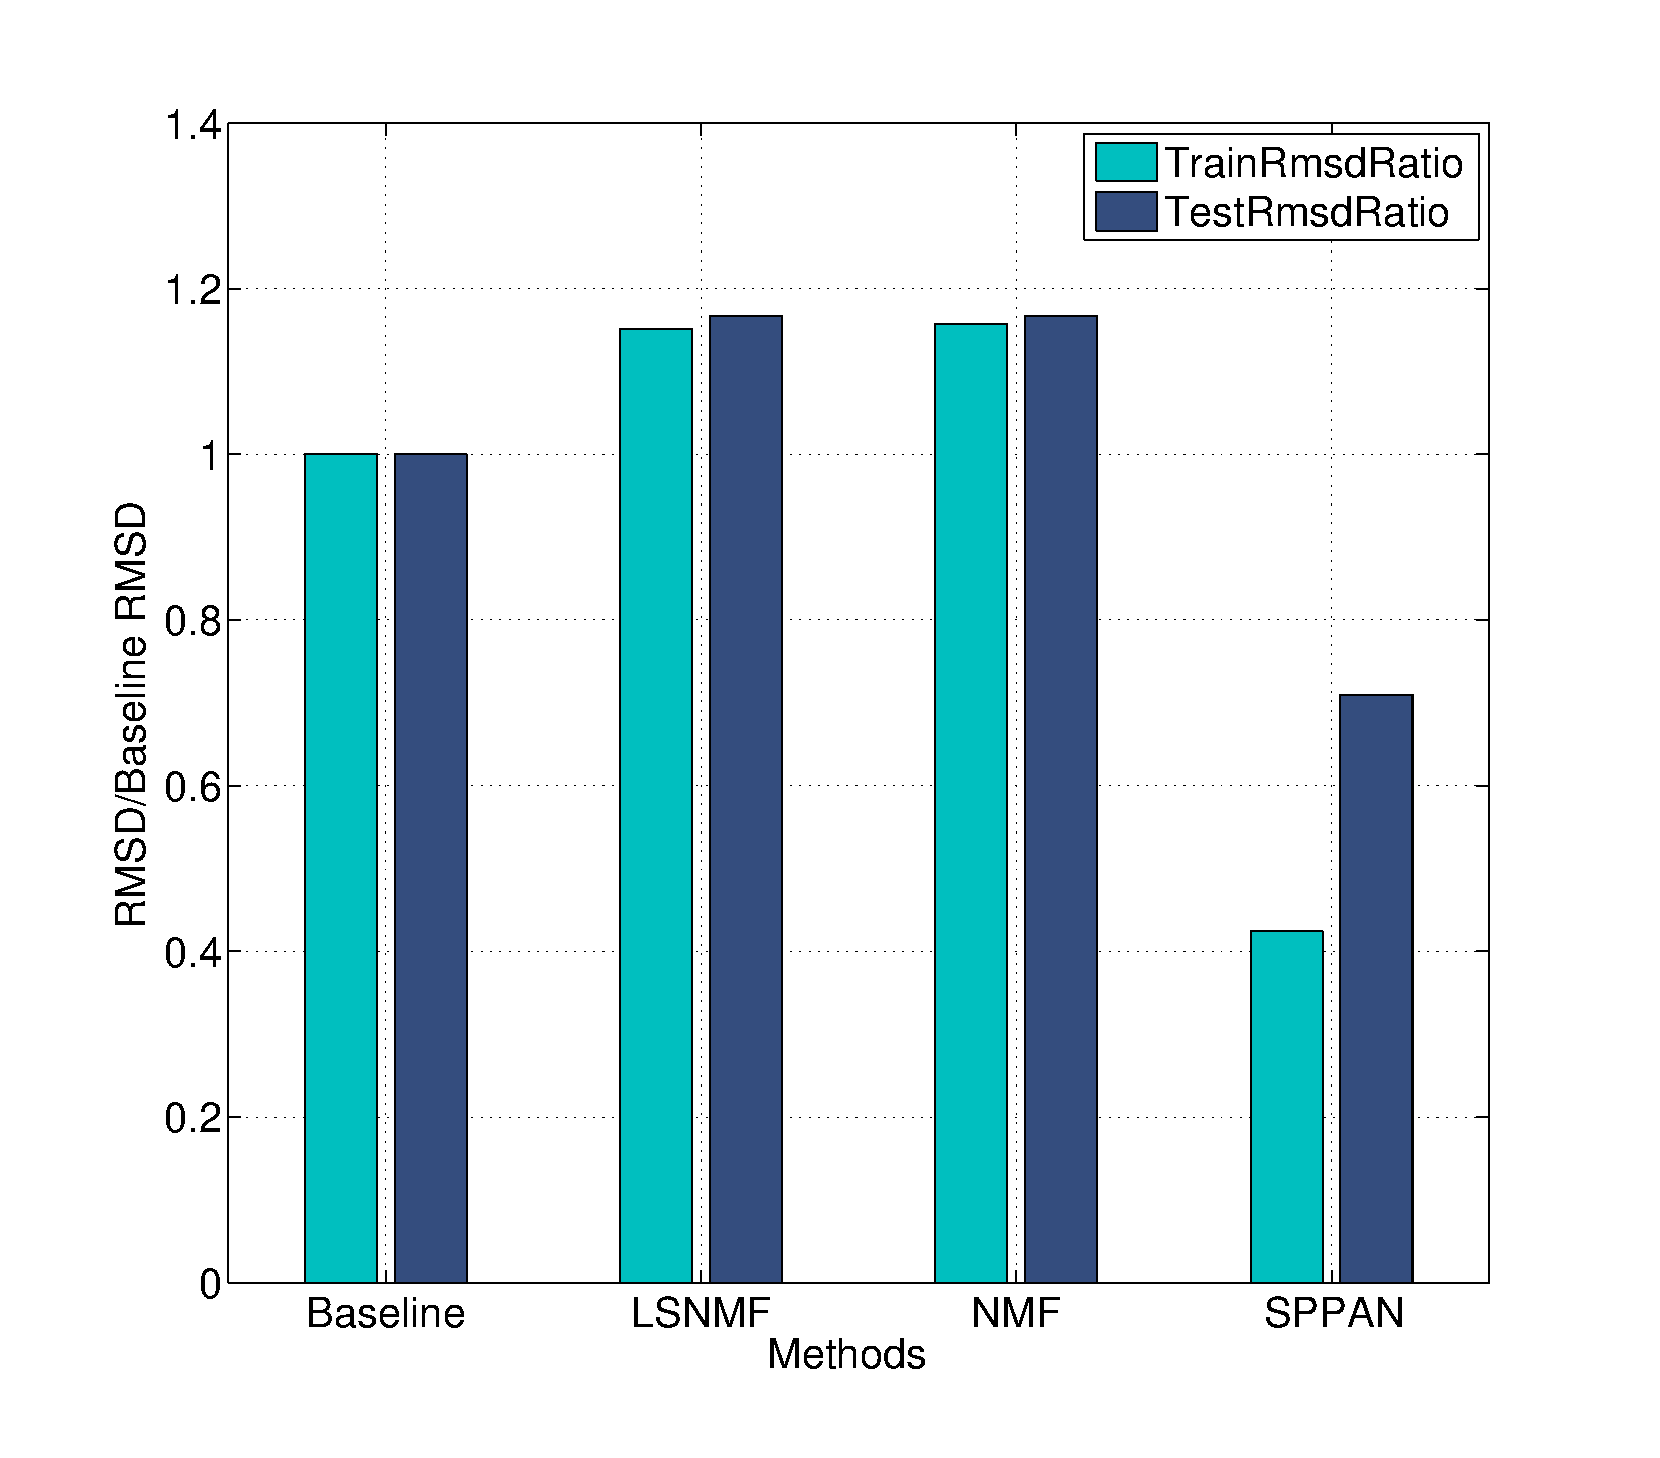
\includegraphics[width=0.45\textwidth]{figures/methos_comparison_all_relative.eps}
  \caption{Compare Relative RMSD Between Different Methods}
  \label{fig:rmsd_compare}
\end{figure}

For a fair comparison with proposed {\sppan} model, we selected the rank
numbers with the best test errors for both LSNMF and NMF. The best
rank numbers for LSNMF and NMF are 3 and 7 respectively.

\begin{table}[!ht]
\centering
\begin{tabular}{|c|c|c|}
  \hline	\hline
  Method &  TrainRmsdRatio&TestRmsdRatio\\ \hline
  Baseline  & $1$  & $1$\\ 
  LSNMF & $1.15$  & $1.17$\\ 
  NMF  & $1.16$  & $1.17$ \\ 
  {\sppan}  & $0.42$  & $0.71$\\ \hline
\end{tabular}
\caption{Relative RMSD in the Best Test Error Round}
\label{tab:rmsd_compare}
\end{table}

Here we list the result relative Root-mean-square deviation(RMSD) of
both training set and testing set from Baseline, LSNMF, NMF and
{\sppan} in Table \ref{tab:rmsd_compare} and Figure
\ref{fig:rmsd_compare} to compare the estimation performance among
these three methods.  The root-mean-square deviation (RMSD) is a
measure of the differences between the estimated value using a model
and the true observed value. It can be expressed using Equation
\ref{eq:rmsd_def}, where $n$ is the number of entries that need be to
estimated, and $\hat{\beta_i}$ and $\beta_i$ are the estimated value
and observed value of entry $i$ respectively. The RMSD represents the
sample standard deviation of the differences between estimated values
and observed values \cite{hyndman2006another}.

\begin{equation}
\label{eq:rmsd_def}
RMSD=\sqrt{\frac{\sum\limits_{i=1}^{n}(\hat{\beta_i}-\beta_i)^2}{n}}
\end{equation}

In order to make those results more meaningful, we use the relative
criteria TrainRmsdRatio and TestRmsdRatio, that are the Train/Test
RMSD of current methods divided by the corresponding RMSD of the
baseline method:
\[
TrainRmsdRatio=\frac{\textit{Train RMSD}}{Baseline Train RMSD}
\]
\[
TestRmsdRatio=\frac{\textit{Test RMSD}}{Baseline Test RMSD}
\]

As can be seen from Figure \ref{fig:rmsd_compare}, even though we
chose the best rank numbers for the Nonnegative Matrix Factorization
based methods, they perform even worse than the baseline method in
this extreme sparse case. {\sppan} model, on the other hand, outperforms
the Baseline, LSNMF and NMF on both training and testing RMSD. To be
more specific, the training and testing RMSD of {\sppan} are only around
$40\%$ and $70\%$ of the training and testing RMSD of Baseline
methods, respectively; they are aroung $35\%$ and $60\%$ of the
training and testing RMSD of the Matrix Factorization based methods
LSNMF and NMF; which shows a great improvement.

\begin{figure}[!ht]
  \centering
  \includegraphics[width=0.42\textwidth]{figures/est_error_hist.eps}
  \caption{Histogram of Estimated Error}
  \label{fig:est_err}
\end{figure}

We also draw the histogram of estimated error generated using {\sppan}
and LSNMF on the testing set as in Figure \ref{fig:est_err}. The
estimated error is defined in Equation \ref{eq:err_def}. For data
privacy considerations, we multiply an constant $k$ in Equation
\ref{eq:err_def}, which doesn't not affect the interpretation of the
following analysis at all. Note that the testing error distribution of
LSNMF and NMF are very similar. Thus we regard the LSNMF result in
Figure \ref{fig:est_err} as the representative result of Nonnegative
Matrix Factorization based method.

\begin{equation}
\label{eq:err_def}
Estimated~Error=k\cdot(Estimated~CTR - True~CTR)
\end{equation}

It can be noticed that the distribution of estimation error of {\sppan}
model is centered on 0 with a normal distribution shape, while LSNMF's
estimation errors are distributed on the left side of 0. It means the
estimations given by LSNMF always have a negative bias which leads to
a constant under-estimation. Therefore, the estimations from the {\sppan}
model is more accurate and reasonable.

\begin{figure}[!ht]
  \centering
  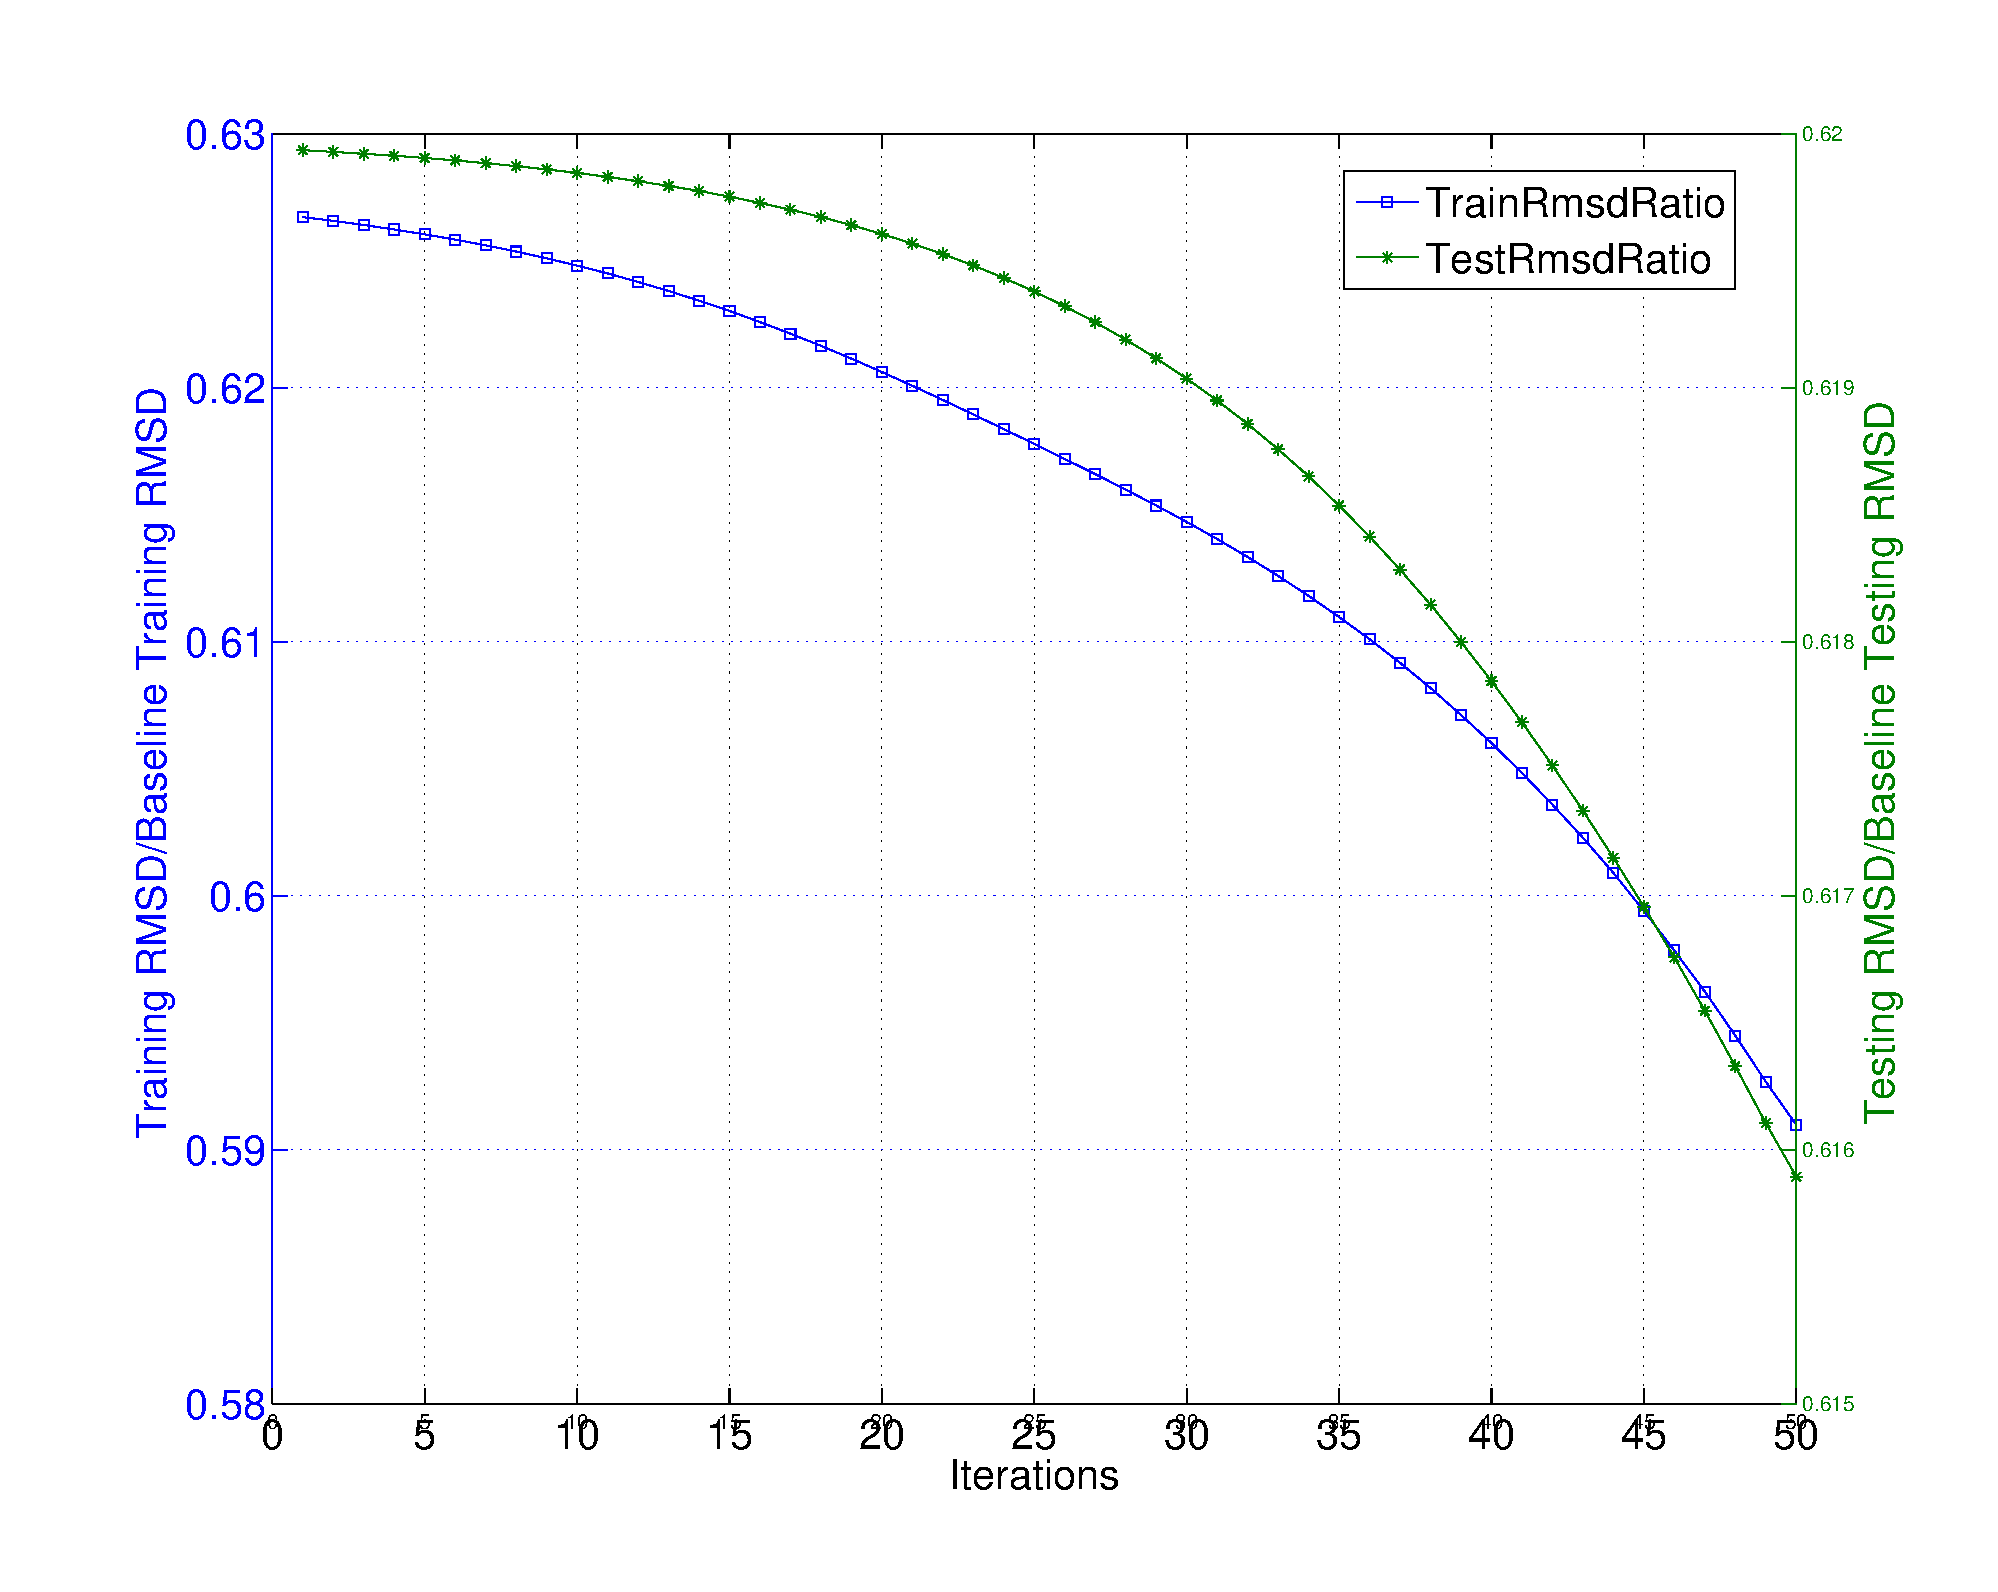
\includegraphics[width=0.42\textwidth]{figures/learning_curve_sppan_whole_relative.eps}
  \caption{{\sppan} Learning Curve on Whole Dataset}
  \label{fig:sppan_curve_whole}
\end{figure}

Besides the experiments on $10\%$ sub sampled data set, it is worth
mentioning that the proposed {\sppan} model can also handle the whole
CTR data set on a single computer. Similar to the model evaluation
experiment on the sub-sampled data set, we separate the whole CTR data
set described in Section \ref{sec:data_desc} into a $95\%$ training
set and a $5\%$ testing set through random selection. Then, we use the
$95\%$ training set to train the {\sppan} model, and test the model on
the $5\%$ testing set. The output training RMSD ratio and testing RMSD
ratio are $0.59$ and $0.62$ respectively, which shows a great
improvement from the baseline method.

We also show the learning curves of {\sppan} model in Figure
\ref{fig:sppan_curve_whole}. It can be seen that both the training
error and testing error were decreasing are decreasing during each
training iterations until the training stop criterion was met, which
is a strong indicator that the {\sppan} model is not over-fitted on the
whole CTR data set.
